\def\thudbabelopt{italian, english}
\documentclass[target=bach, hidelinks]{thud}
\setcounter{tocdepth}{3}
\setcounter{secnumdepth}{3}

\course{Internet of Things, Big Data \& Web}
\title{Feasibility of Electrodermal Activity Data Analysis for Fall Detection using Wearable Devices}
\author{Andrea Cantarutti}
\supervisor{Prof.\ Vincenzo Della Mea}
%\reviewer, \tutor, \chair, \date, \rights

\usepackage[a-1b]{pdfx}
\usepackage[pdfa]{hyperref}

\usepackage{array}
\usepackage{float}
\usepackage{geometry}
\usepackage{minted}
\usepackage{amsmath}
\usemintedstyle{colorful}
\usepackage{eurosym}
\usepackage{subfig}

\begin{document}
\maketitle

\pagestyle{big}

\begin{dedication}

To my mother Clara and my father Dario, \\ whose support and sacrifices led me to reach this milestone. \\
To my beloved Rachele, for always being beside me.
\end{dedication}

\acknowledgements

I would first like to acknowledge my supervisor, Professor Vincenzo Della Mea, for his support and his willingness during my thesis work.

I would also like to express my gratitude to Professor Stefano Fabris from the University of Udine and Jana Schlicksupp from Movisens GmbH, along with all the other people who have contributed to the realisation of this work.

I also wish to thank my fellows Francesco, Lorenzo, Gabriele, Massimiliano and Alessandro, with whom I have had the privilege of sharing the undergraduate experience with enthusiasm and passion.

% \abstract

% Index 
\tableofcontents

\listoftables

\listoffigures

%% Document body (eventually one can use \part{part-name})

\mainmatter

\chapter{Introduction}
\label{section:introduction}

Introduction


\chapter{Background}
\label{ch:background}

In order to define a common ground for the reader, this chapter introduces the main contents on which this work is based. For this purpose, a brief introduction about the current \textbf{state of knowledge} in terms of fall detection and the role of the \textbf{Electrodermal Activity} is proposed. Additionally, the concept of \textbf{Wearable Device} is briefly introduced.

% TODO evaluate the title, might need to be changed
\section{Benefits and Progress of Fall Detection Systems }\label{sec:sectionname}

% file:///Users/andrea/Downloads/sensors-21-05134-v2.pdf
In the field of research, a fall is described as an \textbf{unpredicted event} leading a subject to rest on the floor level~\cite{Lamb1}. On that basis, the activity of Fall Detection has referred over the years to the identification of a fall through cameras and sensors in order to request assistance.

Furthermore, various classifications of falls have been outlined. An accurate set of categories was described by Chan \textit{et al., 2018}~\cite{Chen1}, whose study about the specifications of built-in accelerometers in smartphones on fall detection performance divides falls in the following categories: 

\begin{itemize}
    \item Fall lateral left and lie on the floor
    \item Fall lateral left and sit up from the floor
    \item Fall lateral right and lie on the floor
    \item Fall lateral right and sit up from the floor
    \item Fall forward and lie on the floor
    \item Fall backward and lie on the floor
\end{itemize}

Researchers had also pointed out other important aspects that should be considered while evaluating falls, such as the duration of the fall and the age, gender, mental condition and physical condition of the individual.




\chapter{Modern Approaches for Fall Detection}
\label{ch:fall-detection}

With the purpose of providing a deeper understanding on how some of the most relevant datasets regarding fall detection were collected, an analysis was performed in order to identify common \textbf{patterns}, the \textbf{technologies} employed and the \textbf{results obtained}. 

\section{Typical biometric data employed in fall detection}\label{sec:hardware}

The consequences of falling may be observed through a series of data that addresses aspects related to physical, physiological and environmental variables. Some of the repercussions that a hard fall may cause are:

\begin{itemize}
    \item A fast shift of the gravitational acceleration values
    \item A change of the altitude above ground level
    \item Feelings of fear and obfuscation (especially for elderly people in severe cases)
    \item A decrease of the body temperature (in cases in which the individual remains prone on the ground for extended periods of time)
\end{itemize}

The following section introduces some of the most commonly used instruments to retrieve data that may be functional to fall detection systems.

\subsection{Accelerometer}\label{subsec:accelerometer}

The accelerometer provides a measure of the \textbf{acceleration} in relation to an entity in its coordinate system. Once calibrated, the obtained value measures 9.81 $m/s^2$ at rest (which corresponds to the gravity acceleration) and drops at 0 $m/s^2$ during a \textbf{free fall}.

Furthermore, modern accelerometer are commonly implemented as \emph{micro-electro-mechanical-systems} and their dimensions have packaged sizes of only 2 x 2 x 1 \textit{mm}. This makes them particularly suitable for \textbf{wearable devices} and \textbf{embedded systems}.

Since a 3-axis accelerometer provides a separate trace for the $x$, $y$ and $z$ axis, a \textbf{magnitude vector} can be computed in order to represent the measurement as a scalar value. The formula involves the calculation of the norm of the coordinate vector and is generally computed in real-time on embedded systems in order to provide a value for classification purposes.

\newcommand\norm[1]{\left\lVert#1\right\rVert}

\begin{figure}[h]
    \begin{equation}
    \norm{a}_2 = \sqrt{a_{x}^2 + a_{y}^2 + a_{z}^2}
    \end{equation}
    \caption{Magnitude Vector formula}
    \label{fig:magnitude}
\end{figure}

\subsection{9-Axis IMUs}\label{subsec:imus}

The \textbf{inertial motion sensor} units (commonly referred as IMUs) provide a combination of three sensors:

\begin{itemize}
    \item A 3-axis accelerometer
    \item A 3-axis gyroscope 
    \item A 3-axis magnetometer 
\end{itemize}

While the accelerometer and gyroscope signals provide measures to describe the \emph{rotation} and the \emph{acceleration} around each axis, a magnetometer is employed in order to sense the surrounding \emph{magnetic field} and correct small drifts over long lasting periods of time. 

The combination of the latter sources provides a criteria to compute the \textbf{complete orientation in space} and offers remarkable advantages in order to improve accuracy in motion tracking and fall detection systems.

\subsection{Barometric Altimeter}\label{subsec:altimeter}

The barometric altimeter determines changes in elevation by employing a pressure sensor. Compared to the changes in the atmospheric pressure, in fact, the altitude variation results inversely proportional \cite{mems-altimeter}.

Although barometric altimeters are involved in a multitude of usages, the data collected may provide useful information in the context of fall detection systems. The altitude level, when combined with the data retrieved from a 9-Axis IMU or an accelerometer, may confirm that a fall event just happened with higher levels of accuracy.

Several instruments for motion tracking include both a 9-Axis inertial measurement unit and a barometric altimeter. For that, they are commonly referred as \textbf{10-Axis IMUs}.

\subsection{Biometric Sensors}\label{subsec:biometric-sensors}

Another branch of information which has been widely regarded lately is related to biometric sensors. These include a variety of instruments to collect biometric signals by using appropriate hardware, such as \textbf{electrodes}, \textbf{skin contact technologies} and others.

Besides some units require the usage of specific hardware, other sensors (such as the ECG, EEG, Temperature, EDA and others) have already been implemented in several commercial wearable devices and provide accurate data that can later be involved in the computation of several biometric descriptors. 

In the context of fall detection systems, a synchronized retrieval of both biometric and motion related data may significantly improve the accuracy of classification models.

\section{Multimodal datasets for fall detection systems}\label{sec:datasets}

Despite the fact that various falls datasets have been made available throughout the years, two of them were selected for the purpose of this analysis as a consequence of their relevance in the research environment.

\subsection{UMAFall - A Multisensor Dataset for the Research on Automatic Fall Detection}\label{subsec:umafall}

The \textbf{UMAFall} dataset gained considerable interest since its publication (happened in 2017). The primary difference from other datasets was, in fact, related to the way Casilari \textit{et al., 2018}~\cite{umafall} approached the data collection stage, which involved the usage of multiple units of the same sensor. 

Basing on the conclusions drawn by previous publications, UMAFall was designed in order to provide a public dataset to study the importance of sensor units placement for the effectiveness of fall detection algorithms \cite{umafall}. The traces collected provide measurements of the mobility during daily life activities and falls, obtained by \textbf{five sensing nodes} placed on different positions of the body of several individuals.

\subsubsection{Technologies Involved}\label{subsubsec:umafall-technologies}

The data gathering architecture was implemented as a \textbf{Bluetooth Low Energy} (BLE) piconet composed of:

\begin{itemize}
    \item Four wearable sensors located in four different positions of the body, acting as \textbf{slave nodes}
    \item An Android smartphone, acting as the \textbf{master node}
\end{itemize}

The nodes were implemented through multiple \textbf{SimpleLink SensorTag} units. These consist of IoT devices powered by a CC2650 ARM microcontroller that integrates: 

\begin{itemize}
    \item a 2.4 GHz transceiver
    \item 10 embedded sensors, including an MPU-9250 multichip module
\end{itemize}

The latter made possible the retrieval of motion related data, combining the values registered by a 3-axis gyroscope, a 3-axis accelerometer and a 3-axis magnetometer, which were regularly sent to the master unit and later saved in a CSV file. However, the usage of the Bluetooth protocol has demanded low resolutions in order to avoid saturating the communication channel. Therefore, the \textbf{sample rate} was set to 20 Hz for each unit.

\subsubsection{Activities Performed}\label{subsubsec:umafall-activities}

The four sensors were placed on locations typically reported in literature, such as the ankle, waist, chest and right wrist. Furthermore, the participants consisted of seventeen individuals divided in ten males and seven females aged between 18 and 55 years old.

Because of the practical sensor architecture based on wearable devices, data could be retrieved in a domestic environment and included the activities reported in Table \ref{toc:umafall}

\begin{table}[H]
\centering
\begin{tabular}{ll}
    \hline
    Activity                & Category \\
    \hline
    Body bending            & Daily Activities \\
    Climbing stairs down    & Daily Activities \\
    Hopping                 & Daily Activities \\
    Light jogging           & Daily Activities \\
    Lying down              & Daily Activities \\
    Sitting down            & Daily Activities \\
    Walking                 & Daily Activities \\
    Forward fall            & Fall \\
    Later fall              & Fall \\
    Backwards fall          & Fall \\
    \hline
\end{tabular}
\caption{Activities evaluated in UMAFall}
\label{toc:umafall}
\end{table}

\subsubsection{Results Obtained}\label{subsubsec:umafall-results}

Casilari \textit{et al., 2018}~\cite{umafall} provided a dataset including 531 CSV files of which 322 were reporting daily activities data and 209 were reporting falls related data, each one of 15-seconds duration. An initial analysis was performed in order to describe the variation of the \textbf{Signal Magnitude Vector} for each dataset.

Lastly, the results obtained determined substantial difficulties in distinguishing falls from moderate activities using threshold based techniques. An approach based on the fusion of multiple sensor data and the usage of Machine Learning advances in order to reduce the number of \textbf{false positives} obtained was, lastly, proposed by the authors, but not implemented.

\subsection{UP-Fall Detection Dataset: A Multimodal Approach}\label{sec:upfall}

The \textbf{UP-Fall} dataset was presented in 2019 in order to collect fall-related information according to three major modalities:

\begin{itemize}
    \item \textbf{Wearable sensors}
    \item \textbf{Ambient sensors}
    \item \textbf{Vision devices}
\end{itemize}

The aim of the study was providing a considerable amount of data collected from heterogeneous sources in order to address the lack of publicly available measurements for the evaluation of fall detection systems \cite{upfall}.

\subsubsection{Technologies Involved}\label{subsubsec:upfall-technologies}

The hardware involved consisted of: 

\begin{itemize}
\item Five \textbf{Mbientlab MetaSensor} wearables located in different points of the body and collecting data from: 
    \begin{itemize}
        \item A 3-axis accelerometer
        \item A 3-axis gyroscope
        \item An ambient light sensor
    \end{itemize}
\item A \textbf{NeuroSky MindWave} electroencephalograph headset measuring the brainwave signal
\item Six \textbf{infrared sensors} forming a grid above the floor of the room
\item Two \textbf{Microsoft LifeCam Cinema} cameras providing a frontal and a lateral view of the individual 
\end{itemize}

The data gathering architecture was implemented through the usage of two computers and three Raspberry PI V3 in order to collect the information from all the sensors and later save it in the form of multiple CSV files.

In this case a sample rate of \~ 18.4 Hz was configured in order to accommodate the requirements of all the units involved.

\subsubsection{Activities Performed}\label{subsubsec:upfall-activities}

The UP-Fall dataset was collected in a \textbf{controlled environment} where 17 young and healthy subjects were required to perform 11 different activities with three attempts each \cite{upfall}.

\begin{table}[H]
\centering
\begin{tabular}{ll}
    \hline
    Activity                          &   Category           \\
    \hline
    Walking                           &   Daily Activities   \\
    Standing                          &   Daily Activities   \\
    Sitting                           &   Daily Activities   \\
    Picking up an Object              &   Daily Activities   \\
    Laying                            &   Daily Activities   \\
    Jumping                           &   Daily Activities   \\
    Falling sitting in empty chair    &   Fall               \\
    Falling sideward                  &   Fall               \\
    Falling backwards                 &   Fall               \\
    Falling forwards using knees      &   Fall               \\
    Falling forwards using hands      &   Fall               \\
    \hline
\end{tabular}
\caption{Activities evaluated in UP-Fall}
\label{toc:umafall2}
\end{table}

The raw gathered data was later divided in different time windows and, for each one of them, a \textbf{feature extraction and selection} process was performed. The processed information was, then, used to evaluate the performance of four classification models: 

\begin{itemize}
    \item Random Forest
    \item Support Vector Machines
    \item Multi-Layer Perceptron
    \item \textit{k}-Nearest Neighbors
\end{itemize}

The performances of the latter were evaluated through the metrics of \textit{accuracy}, \textit{precision}, \textit{sensitivity}, \textit{specificity} and $F_1$ - \textit{score}.

A limitation pointed out by the authors \cite{umafall} involves the context of the experimentation: the falls performed were self-initiated and different from real-life falls. These kind of aspects constitute a primary concern for researchers because of the difficulties in addressing them and the inaccuracy they might lead to, as stated in \ref{sec:fallintro}.

\subsubsection{Results Obtained}\label{subsubsec:upfall-results}

The dataset obtained and the following activities of processing and subsequent analysis performed led to observe that the data retrieved from the inertial measurement units of the wearables played a major role in the accuracy of the classification models. The accuracy (depicted by the $F_1$-score) of the IMUs-only based classification reached a value of 70.31\% while classifiers trained with combination of infrared and camera data demonstrated considerably lower performances (between 15\% and 33\%). Lastly, the combination of data collected by wearables, cameras and the EEG sensor obtained the highest $F_1$-score accuracy measure, which corresponded to 70.44\%. 

Additionally, a Convolutional Neural Network was trained in order to improve the classification performance based on video recording data. This reached an $F_1$-\textit{score} of 71.2\%.

In conclusion, in the context of fall detection systems, the analysis performed on the UP-Fall dataset demonstrated that a certain degree of accuracy may be reached by processing data from sources of different nature, even though classifications can be improved by approaching the subject in a multimodal and heterogeneous manner.



\chapter{Electrodermal Activity}
\label{ch:eda-chapter}

The following chapter proposes an in-depth study on the merits of the previously mentioned \textbf{Electrodermal Activity} and its potential implications in the context of fall detection.

% TODO maybe change title
\section{Key Aspects of Skin Conductance Analysis}\label{sec:eda-description}

In the whole field of bio-signals, a subject of interest in the recent years has been the so-called \textbf{Electrodermal Activity}, also known as \textbf{Skin Conductance} or \textbf{Galvanic Skin Response}.

The latter describes the continuous variations of the electrical conductivity of the skin (which is also referred as Skin Conductance or SC) and has been depicted as the main criteria to investigate the psychophysiological states of an individual since the beginning of the 20th century.

\subsection{Correlation with Psychophysiological Stress Detection}\label{subsec:eda-signals}

As stated in section \ref{sec:edaintro}, the Electrodermal Activity provides a non-invasive technique to analyze the activity of the \textbf{Autonomic Nervous System} (ANS) by measuring the resistance opposed by the skin to the electrical current, which varies according to the \textbf{sweat glands} activity.

Perspiration is, in fact, governed by the Sympathetic Nervous System \cite{bartholomew} through the postganglionic sudomotor fibers, in connection with the external stimulations received. On these principles, a situation of emotional distress that induces an excitement of the ANS activity would also cause changes in sweat secretion. The measuring of the latter may, then, provide a qualitative indicator related to the \textbf{emotional response} of a subject \cite{carlson}.

\begin{figure}[h]
    \centering
    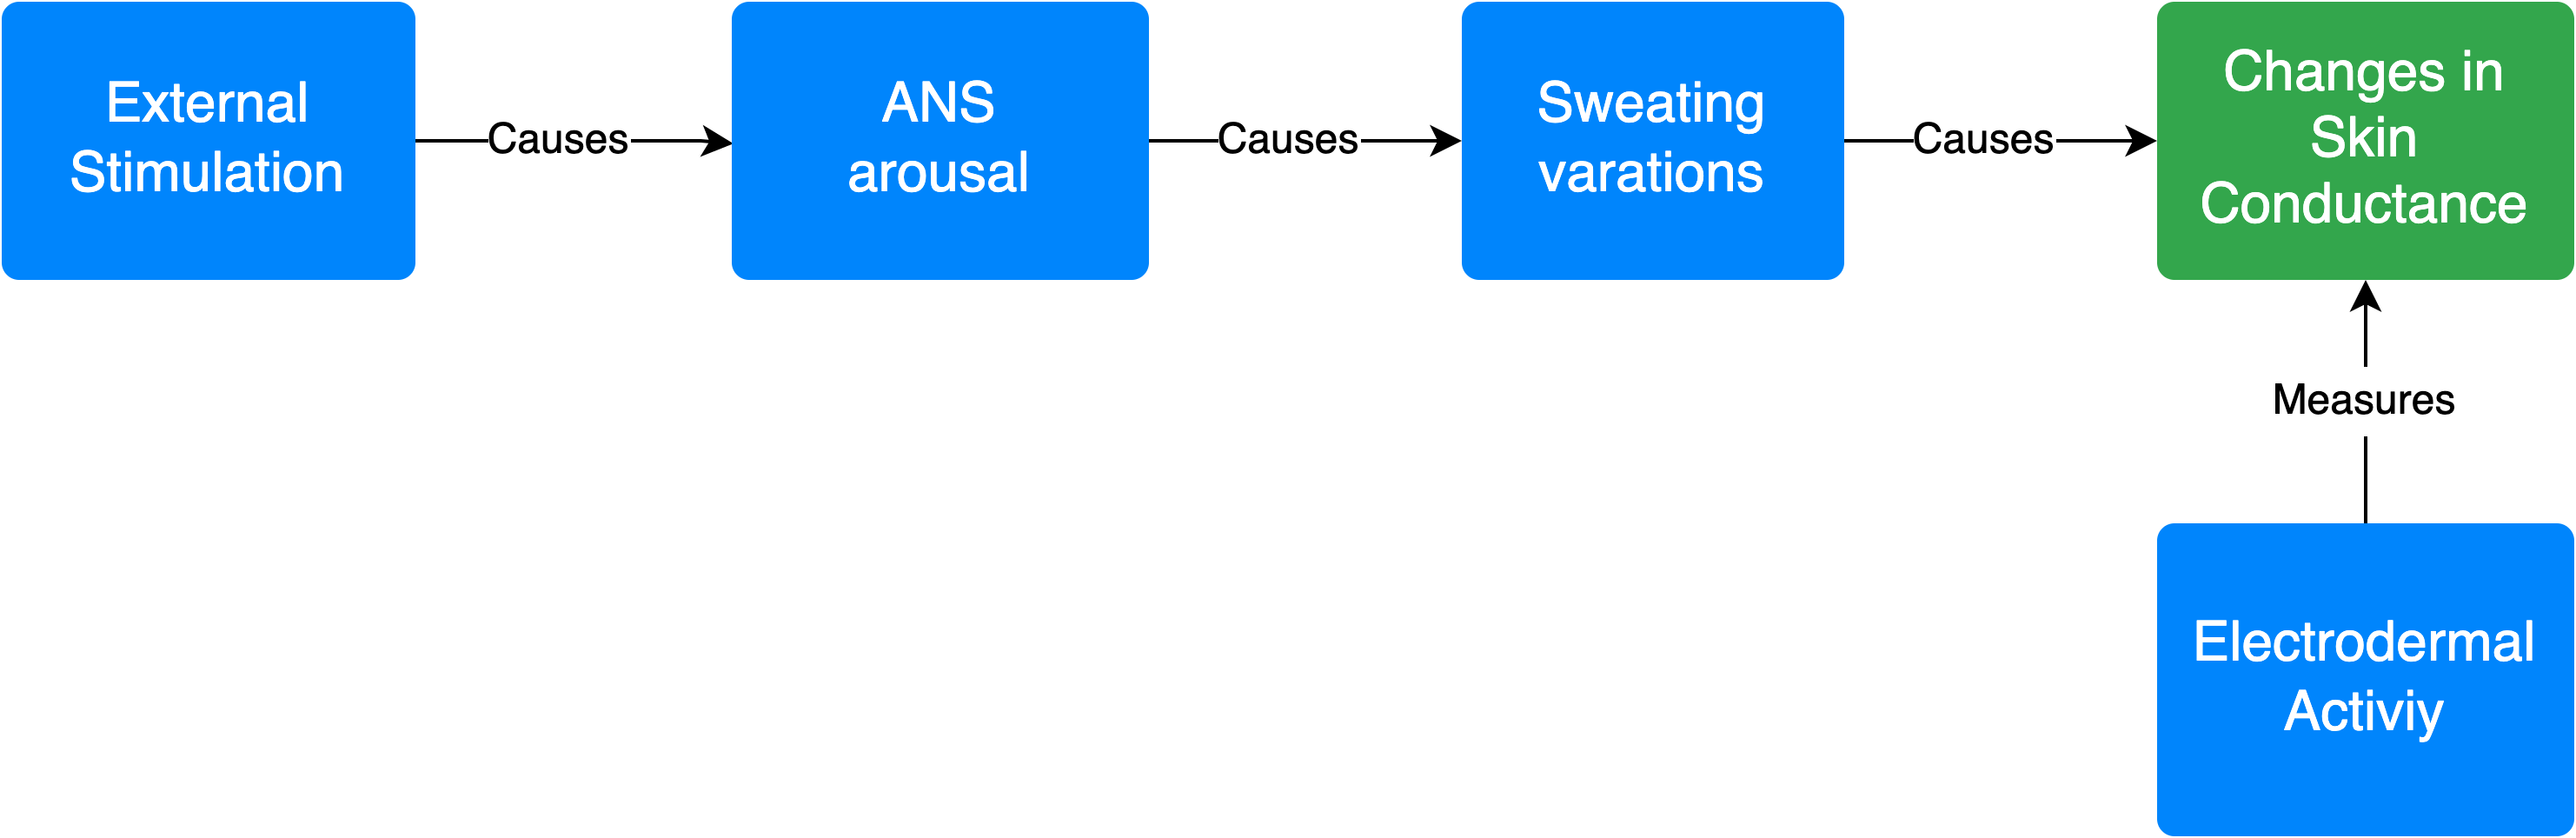
\includegraphics[width=\textwidth]{./images/eda-cause-effect.drawio.png}
    \caption{Correlation between the Electrodermal Activity and the Autonomic Nervous System}
    \label{fig:eda-ans}
\end{figure}

\subsection{Measurement}\label{subsec:eda-measurement}

% https://www.birmingham.ac.uk/Documents/college-les/psych/saal/guide-electrodermal-activity.pdf

In order to detect the Electrodermal Activity on the skin of an individual, two different approaches may be employed:

\begin{itemize}
    \item Exosomatic Methodology
    \item Endosomatic Methodology
\end{itemize}

The first one tends to be the most commonly used and implies the application of a direct or alternating current directly on the skin. The second one, instead, does not involve the usage of any external current.

% https://www.tobiipro.com/learn-and-support/learn/GSR-essentials/how-does-a-gsr-sensor-work/
The implementation of the exosomatic methodology requires the usage of \textbf{two electrodes} through which a voltage of direct current of 0.5 VDC is trasmitted. After being applied to the skin, the current flow through the electrodes is measured by applying the \textbf{Ohm's Law}, which determines the resistance opposed by the epidermis.

\begin{figure}[h]
    \begin{equation}
    \begin{aligned}
    I = \frac{U}{R} \; \; \; \; \; \; \; R = \frac{U}{I}
    \end{aligned}
    \end{equation}
    \caption{Ohm's Law Formula}
    \label{fig:ohmlaw}
\end{figure}

It is important to place both the electrodes on the palm of the hand, on two adjacent fingers or, otherwise, on the sole of the foot. These areas have been, in fact, identified as the most prominent in terms of perspiration. Modern EDA sensors employ electrodes with Ag/AgCl contact points in order to accurately transmit the electrical current \cite{eda-imotions} and isotonic gel is also generally used to accommodate the signal transmission from the skin and consequently improve its quality.

\begin{figure}[h]
    \centering
    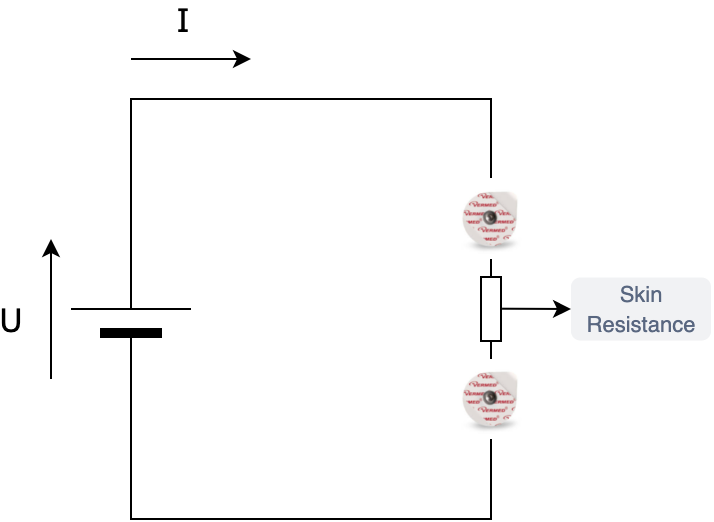
\includegraphics[width=8cm]{./images/skin-resistance.drawio.png}
    \caption{Representation of the EDA measurement principle}
    \label{fig:eda-ans}
\end{figure}

The resistance obtained is expressed in terms of the \textbf{Siemens} ($S$) measuring unit. More specifically, because of the small values obtained, microSiemens ($\mu S$) are normally employed.

\subsection{Sample rates}\label{subsec:eda-signal-properties}

EDA is regarded as a slow measure \cite{eda-guide}. According to the related literature, typical frequency intervals are, in fact:

\begin{itemize}
    \item 0 - 3 Hz \cite{biosignalplux-guide}
    \item 0 - 10 Hz \cite{eda-hci}
    \item 0.0167 - 0.25 Hz \cite{eda-interval-3}
    \item 0.045 - 0.25 Hz \cite{eda-interval-4}
    \item 0.05 - 35 Hz \cite{eda-guide}
\end{itemize}

By applying the \textbf{Nyquist Theorem} \cite{nyquist}, which states that a signal should be sampled at least at two times its highest frequency, it can be inferred that EDA signals must be sampled at 70 Hz or more. In practice, sample rates between 70 Hz and 400 Hz are commonly used according to the requirements of the experimentation in order to provide greater accuracy during the signal processing stage \cite{eda-guide}. Lowpass and bandpass filters are, then, applied in order to smooth the signal and remove unwanted \textbf{noise}.

\subsection{Phasic and Tonic component}\label{subsec:phasic-tonic}

EDA signals are characterized by two \textbf{additive} components \cite{eda-guide} referred as:

\begin{itemize}
    \item \textbf{Tonic component} (also known as Skin Conductance Level or SCL)
    \item \textbf{Phasic component} (also known as Skin Conductance Response or SCR)
\end{itemize}

While the tonic component describes the slowly and continuously changing part of the signal, the phasic component depicts, instead, a fast changing signal whose variations are determined by event-related stimulations.

In order to decompose the measurement obtained in its components, an approach based on \textbf{standard deconvolution} can be employed. Assumed the additivity of the two signals, the skin conductance can be represented as follows:

\begin{equation}
    SC = SC_{tonic} + SC_{phasic}
\end{equation}

Furthermore, both the $SC_{tonic}$ and $SC_{phasic}$ components can be represented by a convolution operation which foresees the multiplication of a so-called \textbf{driver component} recorded by the sensor with an Impulse Response function \cite{edasvm}:

\vspace{5mm}

\begin{figure}[H]
\begin{equation}
SC = Driver_{tonic} \cdot IRF + Driver_{phasic} \cdot IRF
\end{equation}
\caption{Convolution process of the tonic and phasic components}
\label{fig:eda-convolution}
\end{figure}

In order to detect variations in the arousal of an individual over a specific time interval, the phasic component obtained by the deconvolution process is generally employed for feature extraction purposes.

The example reported in Figure \ref{fig:eda-example} illustrates:

\begin{itemize}
    \item A raw EDA signal with a duration of 15 seconds depicting an increase in the arousal level
    \item The subsequently extrapolated SCR component
    \item The SCL component
\end{itemize}

\begin{figure}[h]
    \centering
    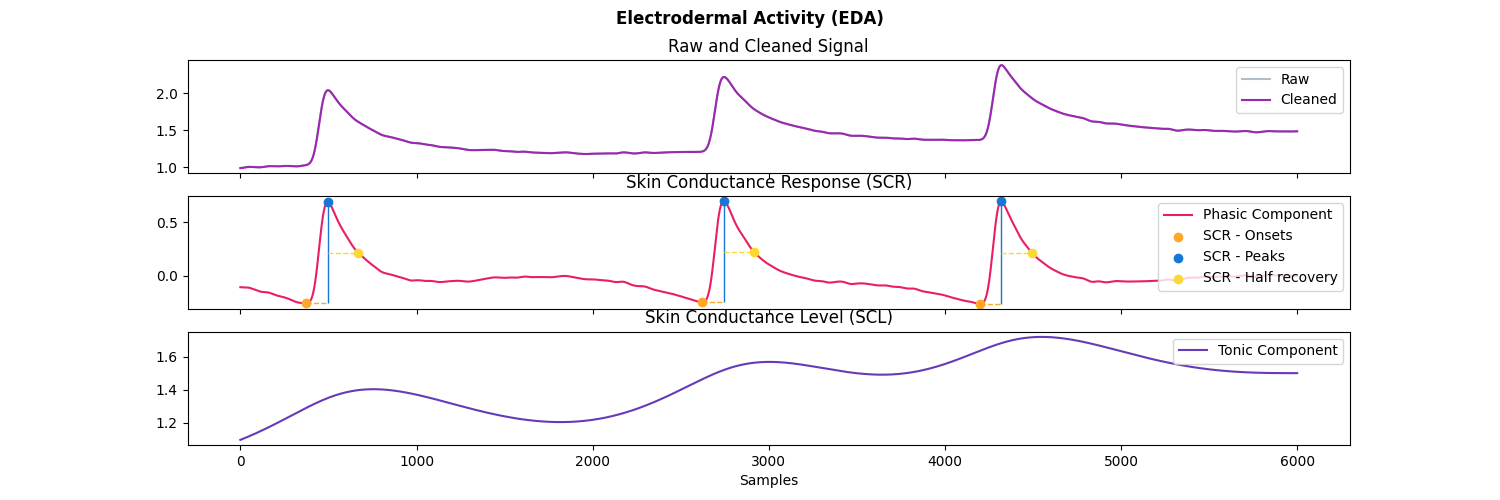
\includegraphics[width=\textwidth]{./images/eda-simulation.png}
    \caption{Decomposition of the raw EDA signal in its two components}
    \label{fig:eda-example}
\end{figure}

The raw signal was generated through \textbf{NeuroKit2}, a Python Toolbox for Neurophysiological Signal Processing that implements several biosignal processing routines, including EDA-related ones \cite{neurokit}.

\subsection{Use Cases}\label{subsec:eda-usecases}

The application of psychophysiological sensors is becoming an increasingly frequent practice in the context of Human Computer Interaction \cite{eda-hci}. More specifically, the Electrodermal Activity may provide a measure that defines the level of \textbf{arousal} that characterizes an individual during experimentations and, generally, the usage of specific technologies.

Recent studies involved, for example, the measurement of both the Heart Rate and the Electrodermal Activity in order to define an objective evaluation method for experiences based on \textbf{virtual reality} \cite{eda-vr}. Moreover, excellent results have been obtained by Sánchez-Reolid \textit{et al., 2018}~\cite{edasvm}, whose classification model based on \textbf{Deep Support Vector Machines} achieved optimal results in the identification of stress patterns by employing EDA measurements acquired from a wearable device.

\section{Electrodermal Activity and Fall Detection Systems}\label{sec:eda-fall-detection}

The Electrodermal Activity measurement in the context of fall detection has not been a true object of interest yet. It is, however, reasonable to assume that analyzing the skin conductance response may provide additional information that helps classifiers reaching higher levels of accuracy. 

In 2013, T. Horta \textit{et al., 2018}~\cite{eda-fall-detection} included EDA signals in the development of a system for fall detection and prevention based on biofeedback monitoring solutions. The latter obtained valid results, but the analysis performed by the authors did not aim to provide assessments on the influence that the Electrodermal Activity had on the accuracy of the whole system (which included other bio-sensors such as electroencephalography, electrocardiogram, electromyography and blood volume pressure).

\subsection{Correlations with Wearable Devices}\label{subsec:eda-wearables}

Because of the nature of EDA signals, during the years the main object of interest has been monitoring patients over extended periods of time and in real-life situations in order to identify patterns that are difficult to replicate in artificial environments. This has consequently focused the interest of researchers on the development of wearable devices for the Electrodermal Activity measurement \cite{poh-wearable}. 

In 2010, Poh \textit{et al., 2018}~\cite{poh-wearable} described one of the first implementations of a compact and cost-effective wearable sensor for unobtrusive and long-term assessment of the Electrodermal Activity. This was packed inside a wristband exposing two electrodes. The outcomes obtained were strongly correlated with FDA-approved measurement systems. Furthermore, over the last decade several companies such as \textbf{Empatica} (an MIT spin-off) or \textbf{Movisens GmbH} (a global leader in ambulatory assessment solutions) implemented highly performing wearable devices for EDA measurement which have been commonly employed in the field of research.

Additionally, at the end of September 2020 \textbf{Fitbit} released \textbf{Sense}, the first commercial wearable device implementing EDA measurement as one of its key features \cite{fitbit-eda}. This opened the way to new opportunities for developers, that will hopefully be able to build software in order to measure and analyse the Electrodermal Activity by employing Application Programming Interfaces of commercial and commonly diffused devices, without having to rely on expensive and invasive equipment.

% Useful? 

% https://www.ncbi.nlm.nih.gov/pmc/articles/PMC2892750/#:~:text=Electrodermal%20activity%20(EDA)%20refers%20to,et%20al.%2C%201981).




\chapter{Implementation of a Wearable Device for High Resolution EDA Logging}
\label{ch:implementation}

Besides the realization of EDA sensors results relatively simple when compared with the circuitry of other devices, its limited diffusion at present implies a series of issues that are required to be addressed. More specifically:

\begin{itemize}
    \item EDA wearables oriented to research purposes tend to be \textbf{particularly expensive} (and most of the time unaffordable for small research projects)
    \item Well-known devices implementing EDA-related features do not provide Application Programming Interfaces for developers and do not provide open-source solutions either
\end{itemize}

The following chapter describes the implementation of a \textbf{simple} and completely \textbf{open-source} wearable device, aimed at providing a low-cost framework for the Electrodermal Activity measurement in \textbf{experimental contexts}.

\section{BITalino Electrodermal Activity Sensor}\label{sec:bitalino}

The sensor unit employed is the purpose-built \textbf{Electrodermal Activity Sensor} by \textbf{BITalino}. This constitutes a single module aimed at composing, along with many others sold by the company, the \textbf{BITalino (r)evolution Board Kit} \cite{bitalino-general}, an all-in-one device implementing a custom firmware for the collection and aggregation of data retrieved from bio-signals. Besides all the features implemented by these boards result interesting in research contexts, the main drawbacks are related to the \textbf{lack of mobility} that the device would cause, which is a primary concern within the bounds of fall detection systems.

Moreover, during the recent years the BITalino EDA module has been employed in a multitude of scientific publications which, overall, have proven that the device allows to reach optimal results in terms of cost-effective Electrodermal Activity analysis.

A \textbf{single EDA module} was purchased for a 25,00 € (Tax Excluded) price and a minimal \textbf{Arduino-based firmware} was implemented in order to retrieve measurements from the individual unit without having to rely on third-party solutions.

\subsection{Description and Features}\label{subsec:bitalino-features}

The EDA sensor module consists of a breakout board whose dimensions correspond to 12mm x 27mm \cite{bitalino-general}. A complete list of informations regarding the configuration of the unit is reported in Table \ref{toc:bitalino-features} .

\begin{table}[H]
\centering
\begin{tabular}{ll}
    \hline
    Parameter               & Value \\
    \hline
    Current                 & DC \\
    Range                   & 0-30 $\mu S$ \\
    Consumption             & $\pm 0.1 mA$ \\
    Bandwidth               & 0 - 2.8 Hz \\
    Measurement             & continuous \\
    Input Voltage Range     & 1.8 - 5.5 V \\
    \hline
\end{tabular}
\caption{Characteristics of the BITalino EDA sensor unit}
\label{toc:bitalino-features}
\end{table}

Furthermore, the device is sold in the three following configurations, according to the requirements of the customers: 
\begin{itemize}
    \item \textbf{Self-assemble}
    \item \textbf{Self-assemble} with \textbf{UC-E6 connectors}
    \item \textbf{Assembled}
\end{itemize}

\vspace{3mm}

The first version consists of the breakout board only and requires manual soldering to obtain a complete configuration. The second one provides, instead, pre-installed UC-E6 connectors in order to facilitate the connection to a BITalino board by using apposite homonymous cables. The assembled version is, lastly, presented as a ready-made configuration that includes: 

\begin{itemize}
    \item Pre-soldered electrodes
    \item Pre-soldered UC-E6 cable
    \item A 3D printed ABS case containing the breakout board
\end{itemize}

% https://bitalino.com/storage/uploads/media/homeguide4-eda.pdf

\subsection{Modifications applied}\label{subsec:bitalno-modifications}

In order to exploit the convenience provided by the case and the pre-soldered electrodes, an \textbf{assembled unit} was acquired and subsequently \textbf{modified} in order to implement the connection with a third-party microcontroller. More specifically, the modification procedure consisted of the following steps: 

\begin{enumerate}
    \item Opening of the ABS case
    \item Desoldering the four UC-E6 connector cables from their respective pins on the breakout board
    \item Soldering a dupont cable on each one of the pins
    \item Widening the cable conduit of the ABS case in order to allow the passage of the previously soldered cables
    \item Closing back the ABS case
\end{enumerate}

The role of the pins provided by the breakout board is depicted by the diagram reported in figure \ref{fig:bitalino-pinmap}

\begin{figure}[h]
    \centering
    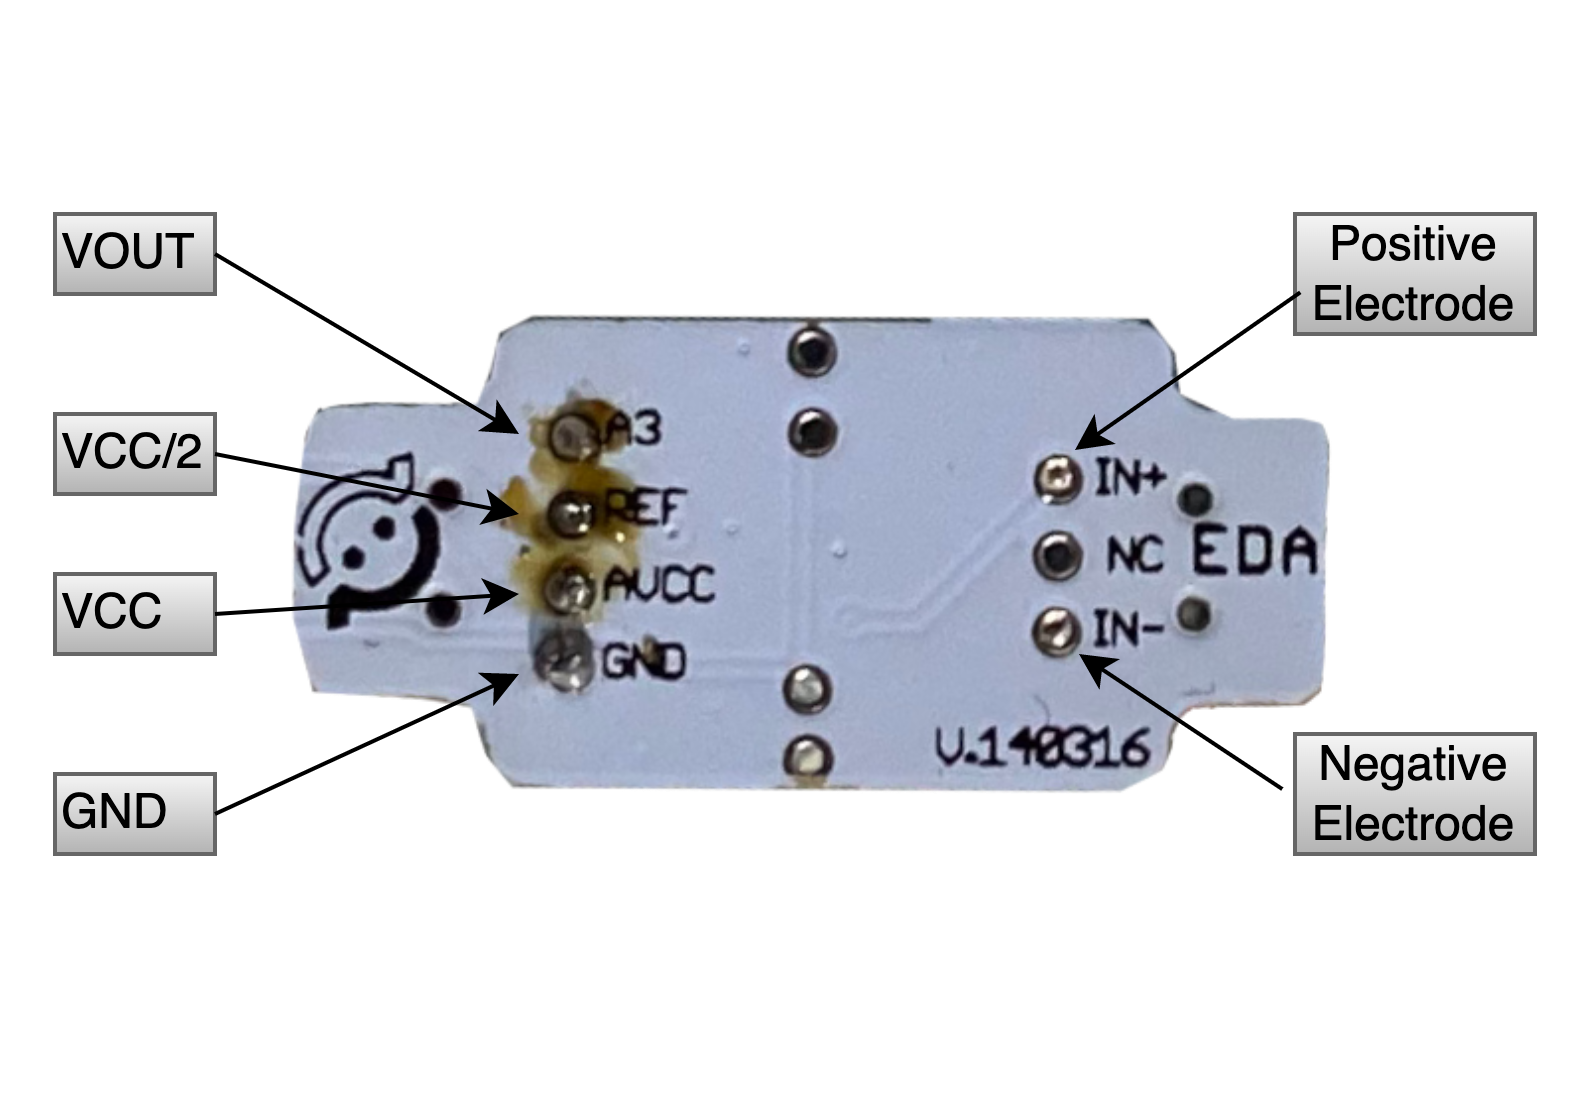
\includegraphics[width=10cm]{./images/bitalino.drawio.png}
    \caption{BITalino EDA sensor pin mapping}
    \label{fig:bitalino-pinmap}
\end{figure}

\vspace{1cm}

More specifically, the function of each pin is reported in table \ref{toc:bitalino-pinmap-table}

\begin{table}[H]
\centering
\begin{tabular}{ll}
    \hline
    \textbf{Pin}            & \textbf{Application} \\
    \hline
    \texttt{IN+}            & Connection input for the positive electrode \\
    \texttt{IN-}            & Connection input for the negative electrode \\
    \texttt{A3}             & Analog output for the EDA signal reading \\
    \texttt{VCC/2}          & Midpoint voltage input, necessary for the microSiemens conversion \\
    \texttt{VCC}            & 3.3 V Voltage input \\
    \texttt{GND}            & Ground input \\
    \hline
\end{tabular}
\caption{Description of the BITalino EDA sensor pin-map}
\label{toc:bitalino-pinmap-table}
\end{table}

\vspace{1cm}

The result obtained after the aforementioned modifications were applied is reported in figure \ref{fig:full-sensor-configuration}. 

It is important to note the role of the \texttt{VCC/2} pin, which permits the flow of a so-called mid-point voltage through the circuit. This provides the necessary \textbf{stability} in order to compute the microSiemens value corresponding to signal measured basing on the output voltage obtained by the sensor \cite{bitalino-midpoint-voltage}. With the aim of providing a correct tension to the \texttt{VCC/2} pin, a voltage divider was implemented by employing two $100 k\Omega$ resistors according to the schematization reported in figure \ref{fig:voltage-divider-schema} . In order to convert the voltage measured by the sensor to the corresponding microSiemens value, the transfer function reported in figure \ref{fig:bitalino-transfer-function} is provided by the official BITalino documentation \cite{bitalino-general}.

\begin{figure}
    \centering
    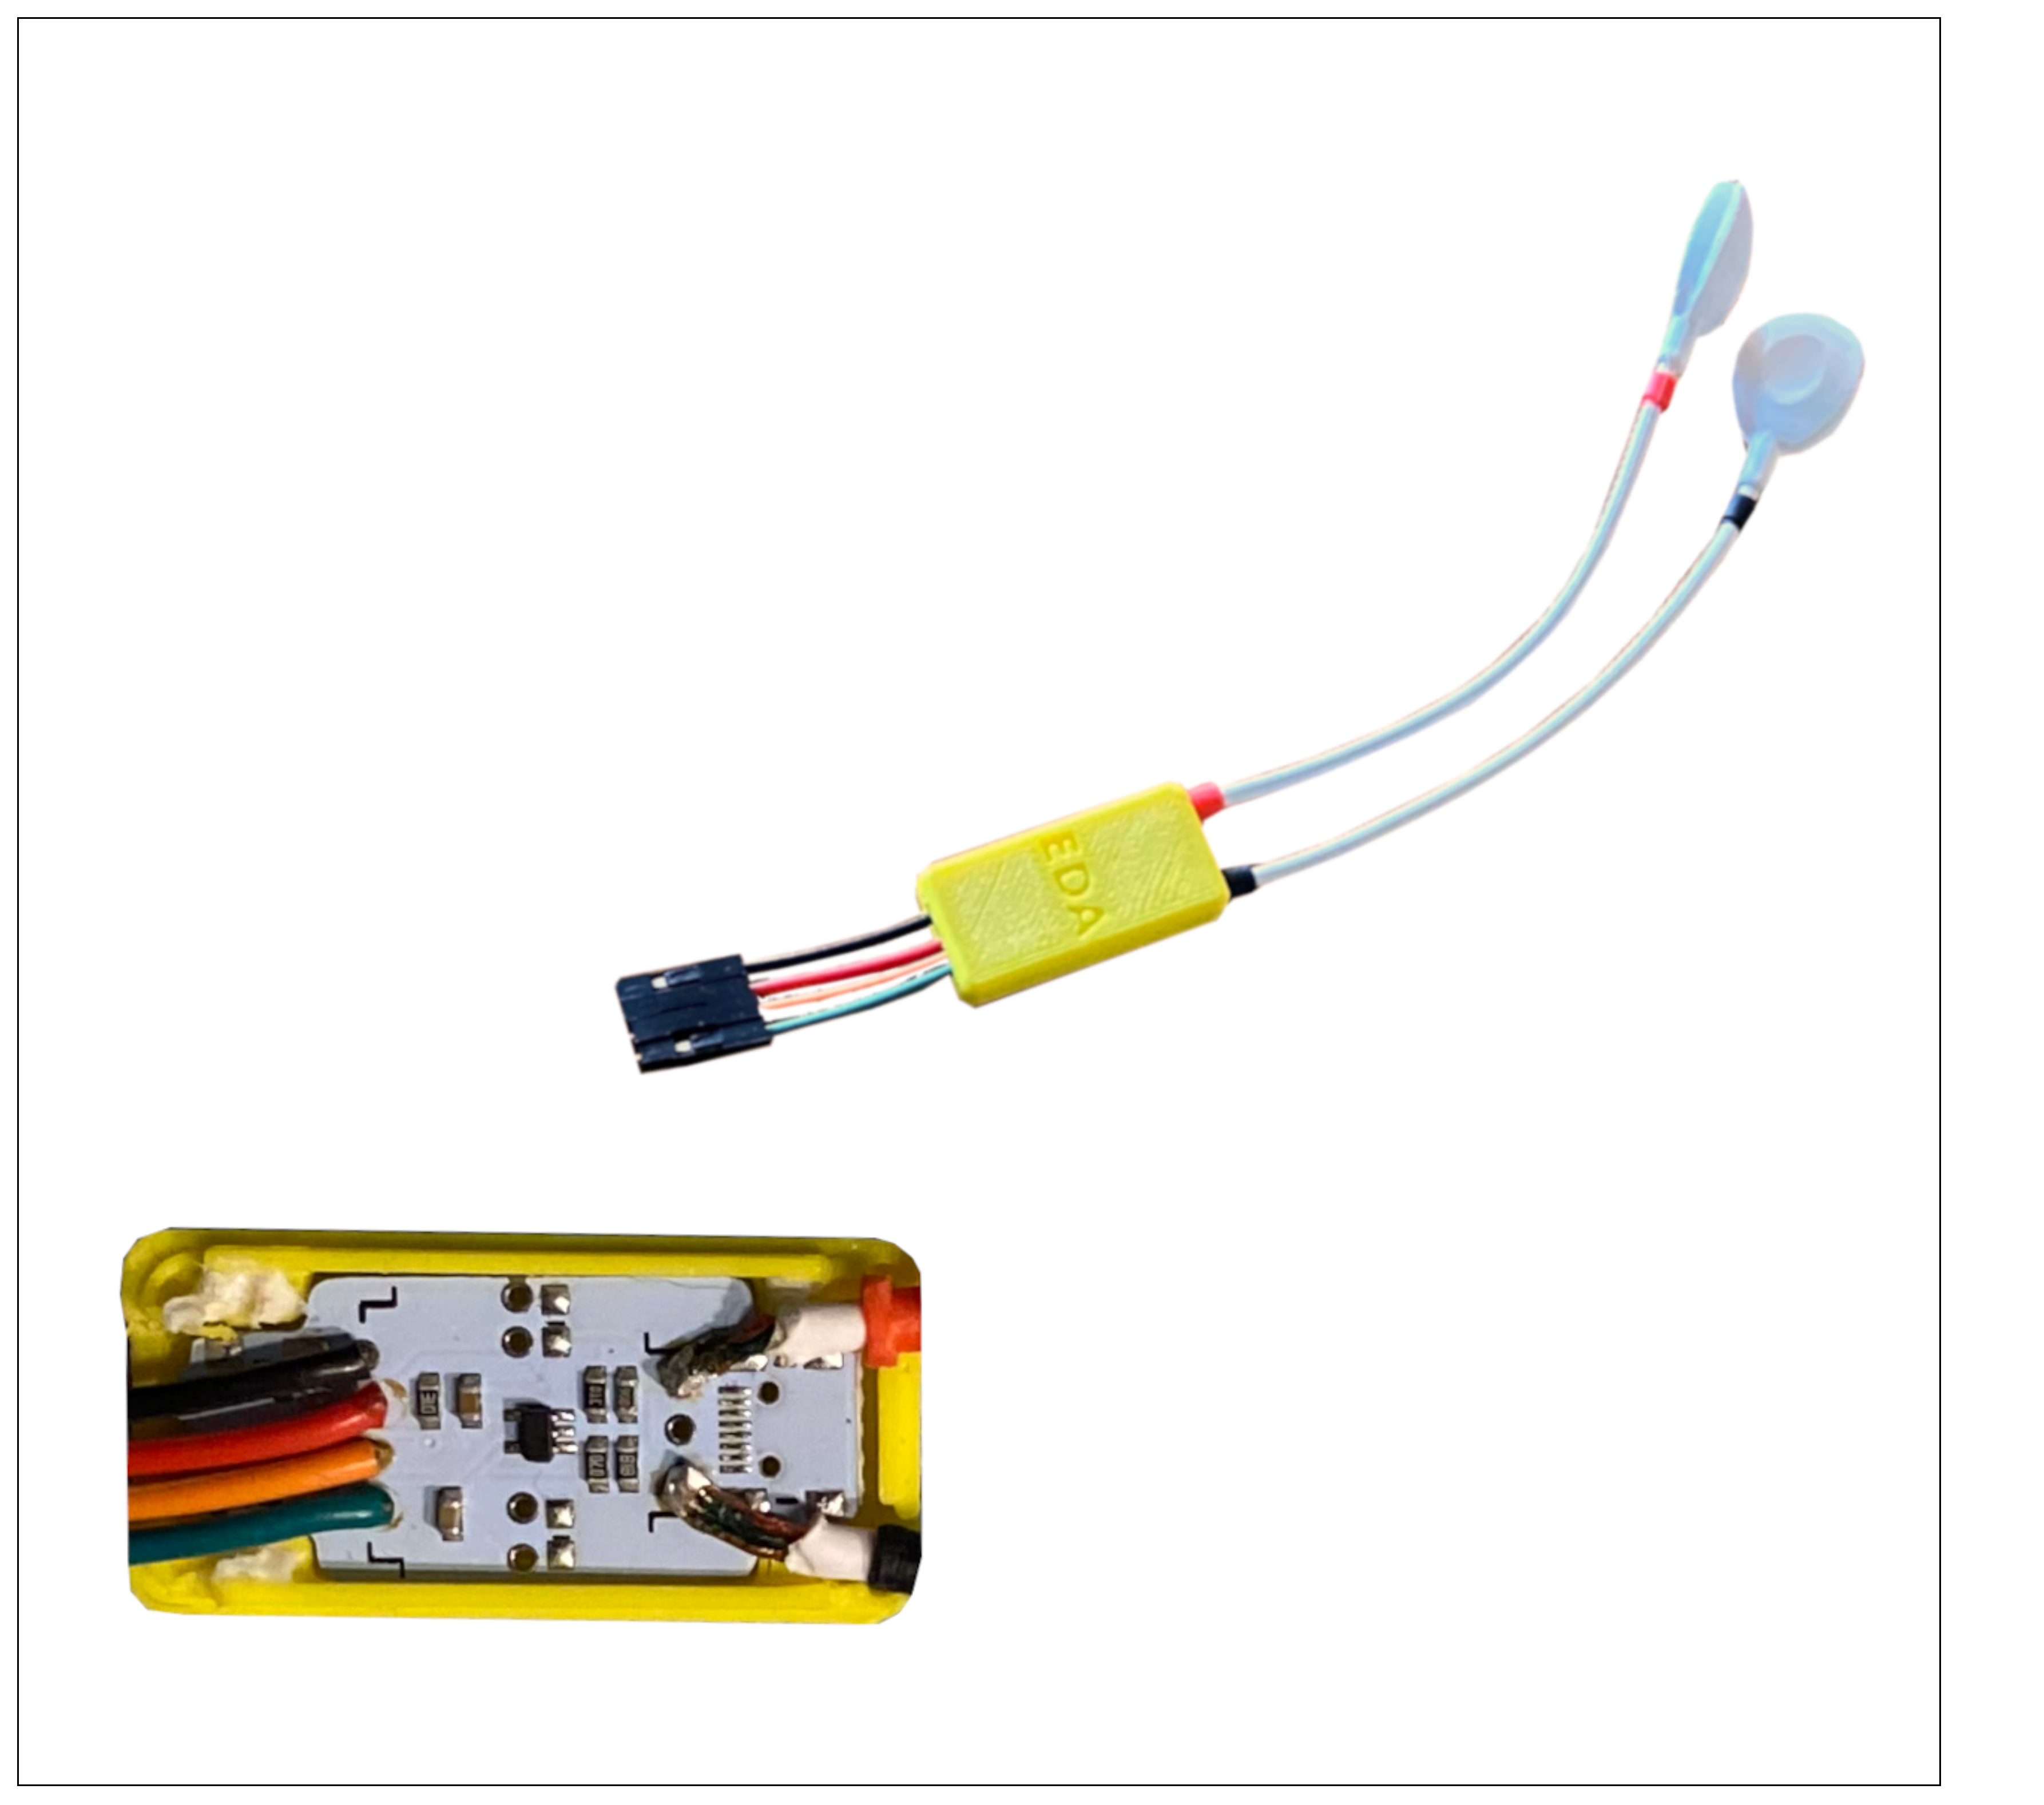
\includegraphics[width=10cm]{./images/full-sensor-view.drawio.png}
    \caption{End result after applying the modifications described}
    \label{fig:full-sensor-configuration}
\end{figure}

\begin{figure}
    \centering
    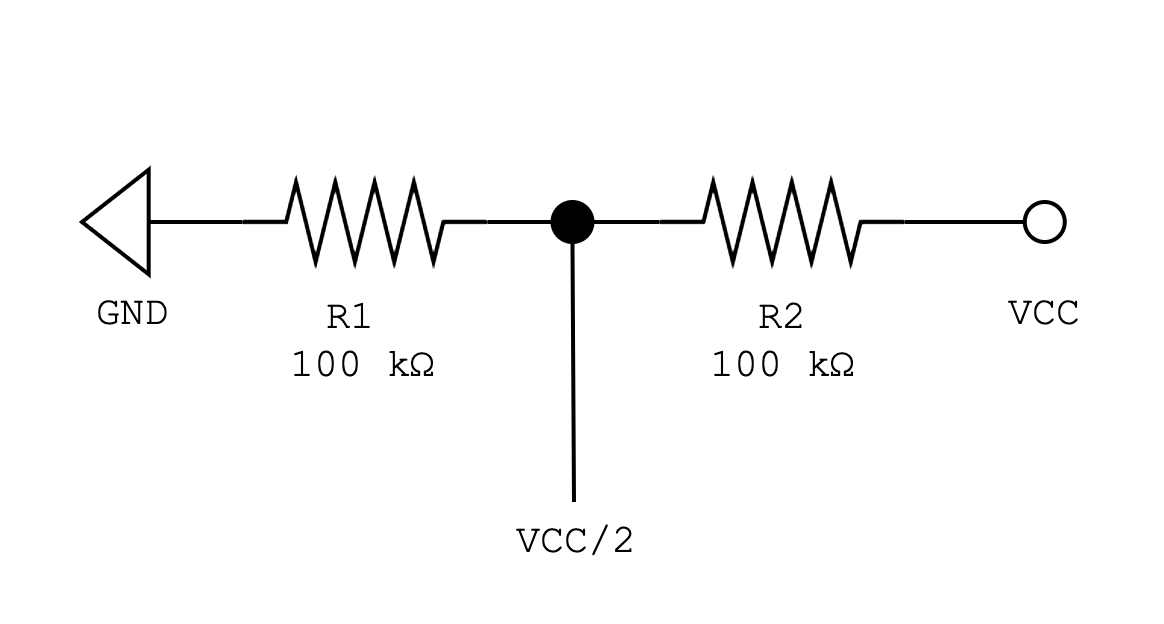
\includegraphics[width=11cm]{./images/midpoint-resistor.drawio.png}
    \caption{Mid-point resistor implemented for the \texttt{VCC/2} pin}
    \label{fig:voltage-divider-schema}
\end{figure}

\begin{figure}
    \begingroup
    \Large
    \begin{equation}
    EDA(\mu S) = \frac{\frac{ADC}{2^n} \cdot VCC}{0.132}
    \end{equation}
    \caption{Transfer function employed for the BITalino EDA sensor}
    \label{fig:bitalino-transfer-function}
    \endgroup
\end{figure}

\pagebreak

\section{Developing a firmware based on the Arduino Framework}\label{sec:firmware}

After applying the necessary changes to the EDA sensor, a research was conducted in order to select an optimal microcontroller upon the following principles: 

\begin{itemize}
    \item Providing a cost-effective solution
    \item Dimensions geared towards high mobility contexts such as fall detection experimentations
    \item Ability to control the system remotely
    \item Limited battery consumption
\end{itemize}

\subsection{Hardware Employed}\label{sec:hardware-employed}

In accordance with the above-stated requirements, a unit based on the well-known \textbf{ESP8266} was employed. The latter consisted, more specifically, of the \textbf{D1 Mini by Wemos} board, which provides easy access to a multitude of functionalities maintaining limited dimensions.

\subsubsection{An overview of the ESP8266}\label{sec:esp8266}

% cite https://en.wikipedia.org/wiki/ESP8266

The ESP8266 consists of an inexpensive 32-bit microcontroller based on the L106 RISC microprocessor that is produced by Espressif Systems. It is widely known and employed in IoT contexts because of its limited dimensions and its native implementation of a full TCP/IP stack, allowing the development of networking-based applications without requiring additional hardware \cite{esp8266}.

Furthermore, the unit exposes 17 GPIO pins which provide a 10-bit resolution analog input and external hardware interfacing through the following protocols:

\begin{itemize}
    \item UART (which allows asynchronous serial communication)
    \item Serial Peripheral Interface (which allows synchronous serial communication)
    \item I$^2$C
    \item I$^2$S
    \item IEEE 802.11 b/g/n
\end{itemize}

Moreover, the ESP8266 offers a capacious flash memory of various Megabytes according to the chosen version and configuration. The latter features allows the indexing of apposite file systems in order to provide persistent memory over restarts. The unit does, though, not provide compatibility with the Bluetooth Low Energy protocol stack (which is a feature that was implemented for the following model, the ESP32).

Additionally, besides Espressif provides its own Software Development Kit (SDK), a multitude of open-source SDKs has been developed over the years. Among all of them, the \textbf{Arduino Framework} stands out because of its accessibility and thanks to the multitude of libraries available. 

\subsubsection{Wemos D1 Mini}\label{subsubsec:d1mini}

For the purposes of this research, a ready-made ESP8266 based board named "Wemos D1 Mini" was employed. The latter provides 16 pins divided into:

\begin{itemize}
    \item 11 digital I/O
    \item 1 analog I/O
    \item 1 RST pin configured for control and reset functions
    \item A single pin for 5V input voltage
    \item A single pin for 3.3V input voltage, which cannot be used together with the 5V one
\end{itemize}

Additionally, the board provides a \textbf{Micro-USB} port which can provide input voltage (substituting the role of the 5V input pin) and data transfer. This allows user to flash compiled binaries to the microcontroller memory in order to execute them. Moreover, since the ESP8266 requires a constant 3.3V input current, the D1 Mini implements a \textbf{voltage regulator} in order to provide the correct internal current, even when the power source provides a voltage above the limit (such as when the unit is powered by a USB cable).

In terms of power consumption, the D1 Mini has a constant drain of 85 mA (which can be reduced drastically when the "Deep Sleep" mode is enabled) and reaches a peak corresponding to 800 mA when powered on.

The figure \ref{fig:d1mini} reports a picture of the D1 Mini unit employed for the experimentation, on which all the pins have been soldered in order to facilitate the test activity by using a breadboard.

\begin{figure}[h]
    \centering
    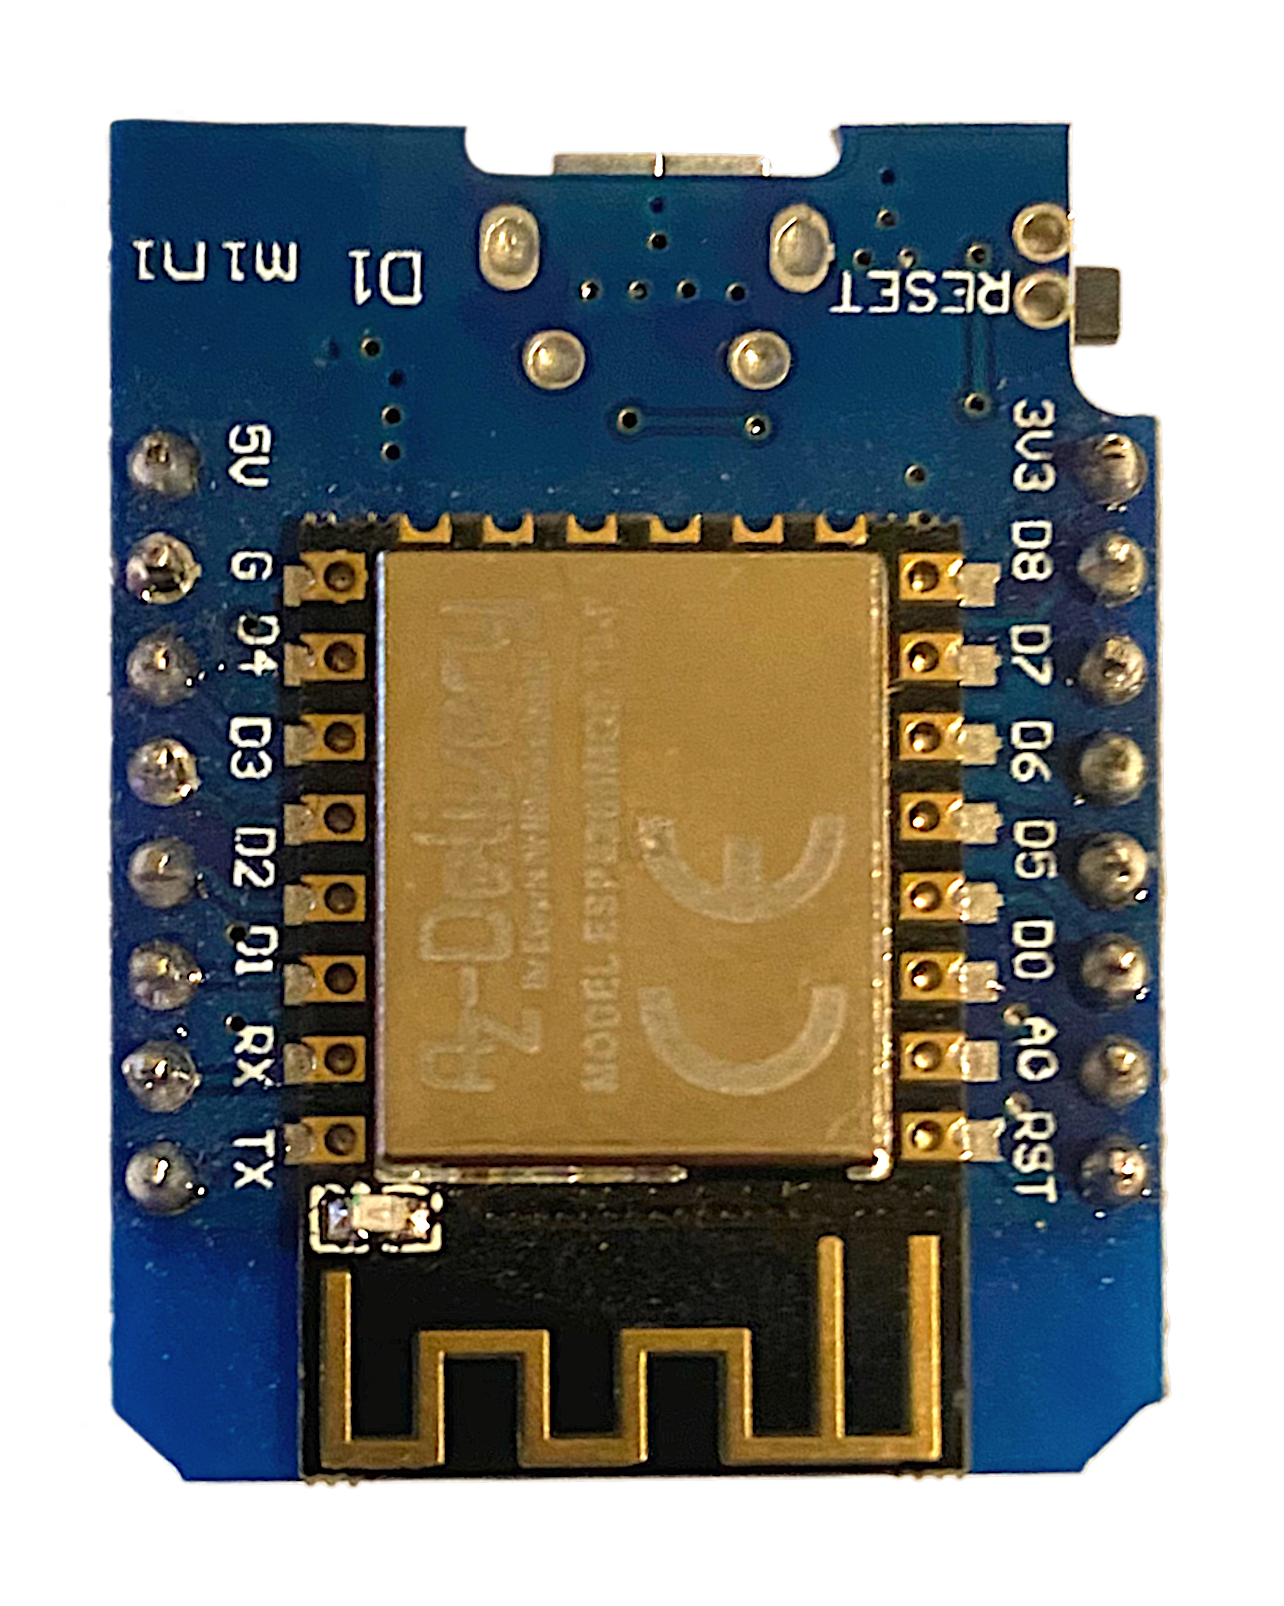
\includegraphics[width=5cm]{./images/d1mini.png}
    \caption{The D1 Mini module employed for the experimentation}
    \label{fig:d1mini}
\end{figure}

\subsubsection{Connection with the BITalino EDA sensor}\label{subsubsec:d1mini}

The modifications applied to the BITalino unit (described in \ref{subsec:bitalno-modifications}) allowed a seamless connection between the D1 Mini and the EDA sensor. The latter was, in fact, directly powered by the microcontroller and connected to its 10-bit resolution analog input. The whole system was, then, powered by a 3.7V-1200mAh Lipo battery. A diagram representing the final circuit is presented in figure \ref{fig:circuit-diagram}

\begin{figure}[h]
    \centering
    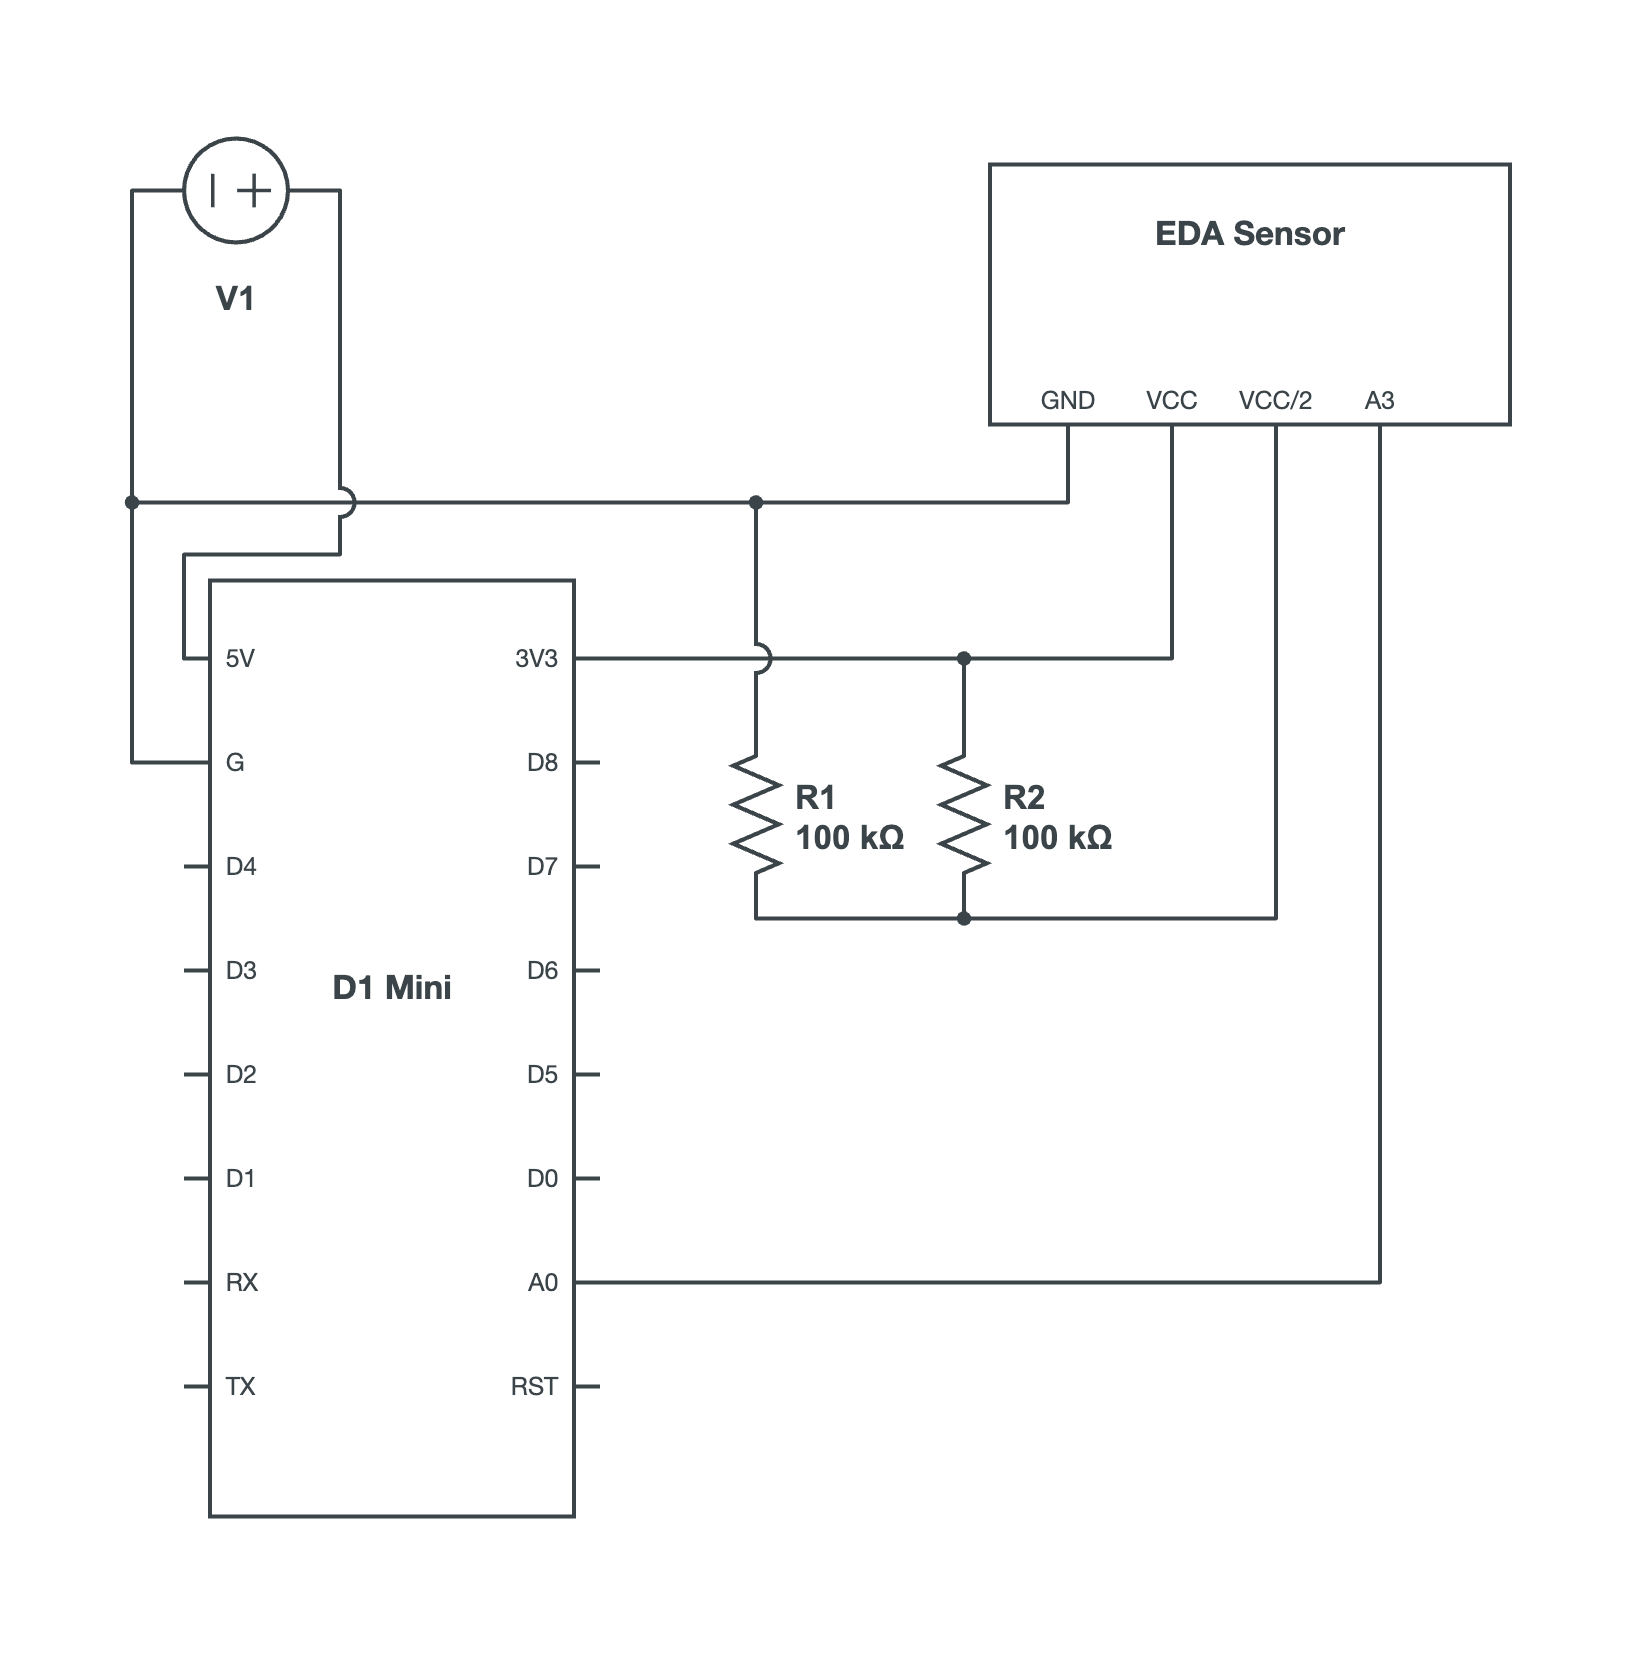
\includegraphics[width=10cm]{./images/circuit-diagram.png}
    \caption{Circuit diagram}
    \label{fig:circuit-diagram}
\end{figure}

The result obtained was finally soldered on a \textbf{matrix board} and packed inside an arm pocket in order to provide protection against the impacts and shocks that a fall may cause.  

\subsection{Firmware Implementation}\label{subsec:firmware-implementation}

As stated previously, the firmware implemented in order to acquire EDA data from the sensor was based on the \textbf{Arduino Framework}, which is at present completely compatible with ESP8266 boards. The latter provides great flexibility and allows easy development for embedded devices. 

The main requirements for the system were the followings:

\begin{itemize}
    \item A functionality that allows the end-user to start each measurement
    \item A functionality that allows to retrieve the measured data
    \item Being able to read data with a sufficiently high sample rate in accordance with the Nyquist Theorem, as stated in \ref{subsec:eda-signal-properties}
\end{itemize}

%IPAddress    apIP(10, 10, 10, 1);                               // Private network address: local & gateway
%
%
%<...>
%void setup() {
%  WiFi.mode(WIFI_AP_STA);
%  WiFi.softAPConfig(apIP, apIP, IPAddress(255, 255, 255, 0));   // subnet FF FF FF 00
%  WiFi.softAP("TardisTime");

In order to address the aforementioned requirements, the device was configured as a \textbf{Soft Access Point} exposing a \textbf{RESTful WebServer} which provides a series of endpoints according to the functionalities required to start each measurement and retrieve the collected data. The EDA activity was sampled at 100 Hz and retrieved from the sensor by employing a logic based on \textbf{Interrupt Service Routines}. The obtained data was, then, buffered and saved on a minimal file system indexed on the flash memory of the microcontroller.

\subsubsection{Libraries Employed}\label{subsubsec:libraries-employed}

In order to exploit the various functionalities required, two additional libraries were included besides the Standard Library that composes the Arduino Framework:

\begin{itemize}
    \item \textbf{LittleFS}
    \item \textbf{ESP8266TimerInterrupt}
\end{itemize}

\textbf{LittleFS} is a library that provides primitives to index and access a file system from the EEPROM (Electrically Erasable Programmable Read-Only Memory) of micro-controllers. It is designed in order to work with limited amounts of storage, providing power-loss resilience and dynamic wear leveling \cite{littlefs}. The latter results fundamental in order to prolong the memory life, which would otherwise be extremely limited in case of micro-controllers. This is made possible be providing a hash-map data structure that maintains a reference for each logical block address that composes the memory space and its current status, in order to select blocks with the lowest erase count for the following write. Furthermore, the library provides functionalities for buffered reading and writing. It was employed in order to gradually save the data retrieved from the EDA sensor in a binary file.

\vspace{8mm}

\textbf{ESP8266TimerInterrupt} enables, instead, the definition of Interrupt Service Routines based on Hardware Timers on ESP8266-based boards \cite{esp8266timerinterrupt}. The latter were employed in order to provide a 100 Hz constant readout from the EDA sensor, by defining a timer that triggers an ISR (which reads data from the sensor and buffers the result) every 10ms.

\vspace{8mm}
A
The firmware was developed in \texttt{C++} using PlatformIO, an open-source framework licensed under the Apache 2.0 license \cite{platformio} which provides several functionalities for embedded development, including scripts for flashing programs to the devices and debug them.

\subsubsection{Program Structure}\label{subsubsec:program-structure}

As required by the Arduino Framework, then program relies on a \mintinline{cpp}{void setup()} function which is executed once everytime the device is started and a \mintinline{cpp}{void loop()} which is, then, executed repeatedly. After including the required libraries, two macro directives were specified in order to indicate the analog pin used for the sensor reading and the sample rate (which is specified in Hz).

\begin{minted}{cpp}
#define EDAPIN A0
#define EDA_SAMPLE_RATE 100
\end{minted}

The main variables and handlers were, then, defined with a global scope. This was performed in order to provide access to:

\begin{itemize}
    \item The \textbf{ESP8266WebServer} handler
    \item The \textbf{ESP8266Timer} handler
    \item The current file descriptor provided by \textbf{LittleFS}
    \item Synchronization flags, declared as \mintinline{cpp}{volatile} when accessed by the Interrupt Service Routine
\end{itemize}

\begin{minted}[frame=single,framesep=10pt]{cpp}
volatile int measurementDuration = 60;
volatile bool measuring = false;
volatile int measurementStart;

IPAddress localIP(192,168,4,22);
IPAddress gateway(192,168,4,9);
IPAddress subnet(255,255,255,0);
ESP8266WebServer server(80);

ESP8266Timer ITimer;

char paramsBuffer[100];
byte payload[12];
File file;
\end{minted}

The setup function configures the WebServer and the Hardware Timer, other than specifying the role of the \texttt{A0} pin. More specifically, the \texttt{/}, \texttt{/start} and \texttt{/retrieve} endpoints are defined in order to respectively acquire informations about the device status, start a measurement for the specified duration and retrieve the previously stored data.

\begin{minted}[frame=single,framesep=10pt]{cpp}
void setup() {
    pinMode(A0, INPUT);

    WiFi.softAPConfig(localIP, gateway, subnet);
    
    if (!WiFi.softAP("eda-measurement", NULL, 1, 0, 1)) {
        Serial.println("Unable to run as Soft Access Point");
        while(1);
    }

    if (!LittleFS.begin()) {
        Serial.println("Unable to run as Soft Access Point");
        while(1);
    }

    ITimer.attachInterrupt(EDA_SAMPLE_RATE, ISRHandler);

    server.on("/", HTTP_GET, info);
    server.on("/start", HTTP_POST, start);
    server.on("/retrieve", HTTP_GET, retrieve);
    server.begin();
}
\end{minted}

More specifically, the \texttt{/start} endpoint starts a measurement for a specified duration and saves the data on a binary file whose name is also specified as a request parameter.

\begin{minted}[frame=single,framesep=10pt]{cpp}
bool initializeNewFile(char *name) {
    return (file = LittleFS.open(name, "w"));
}

void startMeasurement(int durationInSeconds) {
    measurementDuration = durationInSeconds;
    measurementStart = millis();
    measuring = true;
}

void start() {
    const char *args = server.arg("plain").c_str();

    strcpy(paramsBuffer, args);
    char *filename = strtok(paramsBuffer, "|");
    int duration = atoi(strtok(NULL, "|"));

    if (initializeNewFile(filename)) {
        startMeasurement(duration);
        server.send(200, "plain/text", "Starting measurement");
    } else {
        server.send(500, "plain/text", "Unable to initialize a new reading");
    }
}
\end{minted}

The interrupt service routine performs an \mintinline{cpp}{analogRead()} on the EDA sensor pin. Subsequently, the value read from the sensor is combined, together with the one returned by \mintinline{cpp}{millis()}, in a 12-byte payload (using bit-wise operators). The latter is, then, written to the memory as binary data. This is performed by the two following subroutines.

%pagebreak % added to move the whole code block to a new page since the previous one is almost ending

\begin{minted}[frame=single,framesep=10pt]{cpp}

void writeNewDataLine(int sample, long timestamp) {
    payload[0] = (sample >> 24) & 0xFF;
    payload[1] = (sample >> 16) & 0xFF;
    payload[2] = (sample >> 8) & 0xFF;
    payload[3] = sample & 0xFF;  

    payload[4] = (timestamp >> 56) & 0xFF;
    payload[5] = (timestamp >> 48) & 0xFF;
    payload[6] = (timestamp >> 40) & 0xFF;
    payload[7] = (timestamp >> 32) & 0xFF;
    payload[8] = (timestamp >> 24) & 0xFF;
    payload[9] = (timestamp >> 16) & 0xFF;
    payload[10] = (timestamp >> 8) & 0xFF;
    payload[11] = timestamp & 0xFF;

    file.write(payload, 12);
}

void IRAM_ATTR ISRHandler(void) {
    if (measuring) {
        writeNewDataLine(analogRead(EDAPIN), millis());
    }
}
\end{minted}

It is important to note that \mintinline{cpp}{millis()} returns the number of milliseconds elapsed since the microcontroller was powered. Its value was acquired in order to determine the number of milliseconds elapsed between each measurement.

The following subroutine was, instead, defined in order to stop the measurement and save the binary data to the memory storage:

%pagebreak

\begin{minted}[frame=single,framesep=10pt]{cpp}

bool closeFile() {
    if (file) {
        file.close();
        return true;
    }
    return false;
}

bool stop() {
    if (measuring) {
        measuring = false;
        closeFile();
        return true;
    }
    return false;
}
\end{minted}

The \texttt{/retrieve} endpoint was, then, defined in order to send the required binary data as an application/octet-stream mimetype. Once completely streamed to the client, the file is subsequently removed from the memory storage.

\begin{minted}[frame=single,framesep=10pt]{cpp}
void retrieve() {
    String filename = server.arg("plain");
    file = LittleFS.open(filename, "r");

    if (file) {
        server.sendHeader("Content-Type", "text/text");
        server.sendHeader("Content-Disposition", 
                          "attachment; filename=" + filename);
        server.sendHeader("Connection", "close");
        server.streamFile(file, "application/octet-stream");
        file.close();
        LittleFS.remove(filename);
    } else {
        server.send(200, "plain/text", 
                    "Unable to retrieve measurement from memory");
    }
}
\end{minted}

Finally, the \mintinline{cpp}{void loop()} function was configured in order to poll incoming HTTP requests when no measurement is happening or, otherwise, determine when to stop the currently running measurement. This was done with the aim of preventing HTTP requests during a measurement, since both the Wi-Fi antenna and the EDA sensor rely on the same (and only) analog input of the microcontroller.

\begin{minted}[frame=single,framesep=10pt]{cpp}
void loop() {
    if (!measuring) {
        server.handleClient();
    } else {
        const long currentMillis = millis();
        if (currentMillis - measurementStart > measurementDuration * 1000 ) {
            stop();
        }
    }
}
\end{minted}

\pagebreak

\section{Data Collection}\label{sec:data-collection}

% TODO ALTFRAILTY

The device was tested during a session of the \textbf{WP8 ALT-FRAILTY} dataset acquisition. More specifically, the falls reported in table \ref{toc:bitalino-falls} were performed by a 22 years old male volunteer wearing the device on his non-dominant arm.

\vspace{7mm}

\begin{table}[H]
\centering
\begin{tabular}{ll}
    \hline
    Name            &  Description           \\
    \hline
    Rolling         & Falling forward from a chair, landing on the knees \\
    Left Shoulder   & Standing and subsequently falling on the left shoulder \\
    Right Shoulder  & Standing and subsequently falling on the right shoulder \\
    Sidewards       & Standing and subsequently falling sidewards directly on the ground \\
    Bed             & Falling while getting up from the bed \\
    \hline
\end{tabular}
\caption{Falls performed during the first experimentation}
\label{toc:bitalino-falls}
\end{table}



\chapter{Further Investigations}
\label{ch:collection}

%               ROADMAP
% =====================================
%
% we decided to use a commercial product
% movisens and the edamove4
%     - movisens
%     - edamove4
%     - sensor usage and data retrieval
%     - accessory tools
%     - unisens data format
%     - data analyzer and implemented features
% data Collection (falls performed and the hospital context)
% results
%

In order to further investigate the result obtained during the first experimentation session, a second testing trial was performed. This allowed the collection of additional data in order to draw conclusions in relation to the \textbf{feasibility} of the Electrodermal Activity analysis for classification purposes in the context of fall detection.

In this case, a commercial and publicly acknowledged device was employed in order to overcome the issues concerning the sensitivity to shocks and impacts of the BITalino device and, in addition, to acquire further bio-signals along with the Electrodermal Activity data.

\section{Movisens GmbH and the EdaMove Sensor}\label{sec:movisens}

The device employed consists of the \textbf{EdaMove4} sensor by \textbf{Movisens GmbH}, which is one of the most accurate and popular wearable devices aimed at the Electrodermal Activity measurement together with other such as the previously mentioned \textbf{Empatica E4}. Therefore, the following sections propose a brief overview of the product and its features.

\subsection{The company}\label{subsec:movisens-company}


Movisens GmbH is a German company deemed as a global leader in ambulatory assessment solutions \cite{movisens}, which offers several services such as workshops, consults, customized products and software in order to both support researchers and provide technologies and solutions for the healthcare sector.
The current catalog offers several sensor units for data collection and different mobile and desktop applications for data integration, processing and analysis. More specifically, the table \ref{toc:movisens-products} provides a list of the current available products.

\begin{table}[H]
\centering
\begin{tabular}{ll}
    \hline
    Name                     &  Description \\
    \hline
    \textbf{Move 4}          & A 10-Axis IMU that integrates a temperature sensor \\
    \textbf{EcgMove 4}       & A Move 4 unit that integrates ECG data collection  \\
    \textbf{EdaMove 4}       & A Move 4 unit that integrates EDA data collection \\
    \textbf{LightMove 4}     & A Move 4 unit that integrates the acquisition of ambient light measurements \\
    \textbf{SensorTrigger}   & A mobile solutions for activity-triggered data logging \\
    \textbf{movisensXS}      & A mobile solutions for Experience Sampling purposes \\
    \textbf{DataMerger}      & A desktop-based application for the integration of heterogeneous data \\
    \textbf{DataAnalyzer}    & A desktop-based application to analyze and report the acquired data \\
    \textbf{Unisens Viewer}  & A desktop-based application to examine the acquire data \\
    \hline
\end{tabular}
\caption{List of products offered by Movisens GmbH}
\label{toc:movisens-products}
\end{table}

Moreover, the company provides several solutions that allow researchers and students to utilize the needed instrumentation by requiring a free, limited rent for a specific product. In this case, the company has consented a rental related to the \textbf{EdaMove 4} sensor for the required period of time. 

\subsection{The EdaMove 4 Sensor}\label{subsec:edamove4}





\chapter{Conclusions}
\label{ch:conclusions}

This dissertation aimed to provide an assessment related to the feasibility of the Electrodermal Activity data analysis in the context of fall detection. For this purpose, the concepts of \textbf{Skin Conductance} and \textbf{Wearable Devices}, as well as the most important aspects of fall detection systems were briefly introduces and later examined. More specifically, the common technologies employed in the context of fall detection were described and some of the most relevant results in the field of research were, then, analyzed. Afterwards, a description regarding the nature of the \textbf{Electrodermal Activity signals} and their characteristics was provided, together with a careful analysis related to the implications of the Skin Conductance in research contexts.

The approach adopted for the implementation of a Wearable Device aimed at providing high resolution EDA data logging was then described. For this purpose, after an analysis related to the features of the \textbf{BITalino EDA Sensor}, the hardware and software choices made in order to provide a simple and practical implementation were outlined. The device was tested and validated in an apposite experimental context. Besides issues related to its frailty were identified, a first data retrieval session was possible. A subsequent analysis of the collected EDA data was proposed and the results obtained suggested the need of further investigations in order to assess possible correlation between the Electrodermal Activity and fall detection.

Thanks to the collaboration of the \textbf{Movisens GmbH} German company, a high-end wearable device rented in order to collect additional data in a second experimental session. Several falls were performed and the retrieved data was later processed and analyzed.

Besides typical EDA features have been detected during the overall measurement, the results obtained have not demonstrated a clear correlation with the falling activities performed by the participant involved in the experimentation. Moreover, the acquired signal was strongly influenced by motion artifacts which did not allow a clean data collection. For this purpose, better processing technologies (such as specific filters) and acquisition criteria should be provided in order to allow the assessment of the Electrodermal Activity even in contexts of high mobility.

Finally, the observation of specific data acquired during the falls examined suggested that an extensive analysis related to the Electrodermal Activity measurement during \textbf{unexpected falls} should be addressed. In fact, self initiated and simulated falls may be cause of psychophysiological reactions that differ from the ones observable in real-life scenarios. However, obtaining these kind of data at present results considerably difficult because of \textbf{economical}, \textbf{practical} and \textbf{ethical reasons}.

Hopefully, this work will help researchers with the intent of providing further acquisitions of the Electrodermal Activity data in order to configure experimentations aimed at capturing bio-signals similar to the ones that would be retrieved in uncontrolled environments.




\backmatter

% A summary can be added with \summary

\bibliography{thud}
\bibliographystyle{plain_\languagename}

\end{document}

